% Options for packages loaded elsewhere
\PassOptionsToPackage{unicode}{hyperref}
\PassOptionsToPackage{hyphens}{url}
\PassOptionsToPackage{dvipsnames,svgnames,x11names}{xcolor}
%
\documentclass[
  letterpaper,
  DIV=11,
  numbers=noendperiod]{scrartcl}

\usepackage{amsmath,amssymb}
\usepackage{lmodern}
\usepackage{iftex}
\ifPDFTeX
  \usepackage[T1]{fontenc}
  \usepackage[utf8]{inputenc}
  \usepackage{textcomp} % provide euro and other symbols
\else % if luatex or xetex
  \usepackage{unicode-math}
  \defaultfontfeatures{Scale=MatchLowercase}
  \defaultfontfeatures[\rmfamily]{Ligatures=TeX,Scale=1}
\fi
% Use upquote if available, for straight quotes in verbatim environments
\IfFileExists{upquote.sty}{\usepackage{upquote}}{}
\IfFileExists{microtype.sty}{% use microtype if available
  \usepackage[]{microtype}
  \UseMicrotypeSet[protrusion]{basicmath} % disable protrusion for tt fonts
}{}
\makeatletter
\@ifundefined{KOMAClassName}{% if non-KOMA class
  \IfFileExists{parskip.sty}{%
    \usepackage{parskip}
  }{% else
    \setlength{\parindent}{0pt}
    \setlength{\parskip}{6pt plus 2pt minus 1pt}}
}{% if KOMA class
  \KOMAoptions{parskip=half}}
\makeatother
\usepackage{xcolor}
\setlength{\emergencystretch}{3em} % prevent overfull lines
\setcounter{secnumdepth}{5}
% Make \paragraph and \subparagraph free-standing
\ifx\paragraph\undefined\else
  \let\oldparagraph\paragraph
  \renewcommand{\paragraph}[1]{\oldparagraph{#1}\mbox{}}
\fi
\ifx\subparagraph\undefined\else
  \let\oldsubparagraph\subparagraph
  \renewcommand{\subparagraph}[1]{\oldsubparagraph{#1}\mbox{}}
\fi

\usepackage{color}
\usepackage{fancyvrb}
\newcommand{\VerbBar}{|}
\newcommand{\VERB}{\Verb[commandchars=\\\{\}]}
\DefineVerbatimEnvironment{Highlighting}{Verbatim}{commandchars=\\\{\}}
% Add ',fontsize=\small' for more characters per line
\newenvironment{Shaded}{}{}
\newcommand{\AlertTok}[1]{\textcolor[rgb]{1.00,0.33,0.33}{\textbf{#1}}}
\newcommand{\AnnotationTok}[1]{\textcolor[rgb]{0.42,0.45,0.49}{#1}}
\newcommand{\AttributeTok}[1]{\textcolor[rgb]{0.84,0.23,0.29}{#1}}
\newcommand{\BaseNTok}[1]{\textcolor[rgb]{0.00,0.36,0.77}{#1}}
\newcommand{\BuiltInTok}[1]{\textcolor[rgb]{0.84,0.23,0.29}{#1}}
\newcommand{\CharTok}[1]{\textcolor[rgb]{0.01,0.18,0.38}{#1}}
\newcommand{\CommentTok}[1]{\textcolor[rgb]{0.42,0.45,0.49}{#1}}
\newcommand{\CommentVarTok}[1]{\textcolor[rgb]{0.42,0.45,0.49}{#1}}
\newcommand{\ConstantTok}[1]{\textcolor[rgb]{0.00,0.36,0.77}{#1}}
\newcommand{\ControlFlowTok}[1]{\textcolor[rgb]{0.84,0.23,0.29}{#1}}
\newcommand{\DataTypeTok}[1]{\textcolor[rgb]{0.84,0.23,0.29}{#1}}
\newcommand{\DecValTok}[1]{\textcolor[rgb]{0.00,0.36,0.77}{#1}}
\newcommand{\DocumentationTok}[1]{\textcolor[rgb]{0.42,0.45,0.49}{#1}}
\newcommand{\ErrorTok}[1]{\textcolor[rgb]{1.00,0.33,0.33}{\underline{#1}}}
\newcommand{\ExtensionTok}[1]{\textcolor[rgb]{0.84,0.23,0.29}{\textbf{#1}}}
\newcommand{\FloatTok}[1]{\textcolor[rgb]{0.00,0.36,0.77}{#1}}
\newcommand{\FunctionTok}[1]{\textcolor[rgb]{0.44,0.26,0.76}{#1}}
\newcommand{\ImportTok}[1]{\textcolor[rgb]{0.01,0.18,0.38}{#1}}
\newcommand{\InformationTok}[1]{\textcolor[rgb]{0.42,0.45,0.49}{#1}}
\newcommand{\KeywordTok}[1]{\textcolor[rgb]{0.84,0.23,0.29}{#1}}
\newcommand{\NormalTok}[1]{\textcolor[rgb]{0.14,0.16,0.18}{#1}}
\newcommand{\OperatorTok}[1]{\textcolor[rgb]{0.14,0.16,0.18}{#1}}
\newcommand{\OtherTok}[1]{\textcolor[rgb]{0.44,0.26,0.76}{#1}}
\newcommand{\PreprocessorTok}[1]{\textcolor[rgb]{0.84,0.23,0.29}{#1}}
\newcommand{\RegionMarkerTok}[1]{\textcolor[rgb]{0.42,0.45,0.49}{#1}}
\newcommand{\SpecialCharTok}[1]{\textcolor[rgb]{0.00,0.36,0.77}{#1}}
\newcommand{\SpecialStringTok}[1]{\textcolor[rgb]{0.01,0.18,0.38}{#1}}
\newcommand{\StringTok}[1]{\textcolor[rgb]{0.01,0.18,0.38}{#1}}
\newcommand{\VariableTok}[1]{\textcolor[rgb]{0.89,0.38,0.04}{#1}}
\newcommand{\VerbatimStringTok}[1]{\textcolor[rgb]{0.01,0.18,0.38}{#1}}
\newcommand{\WarningTok}[1]{\textcolor[rgb]{1.00,0.33,0.33}{#1}}

\providecommand{\tightlist}{%
  \setlength{\itemsep}{0pt}\setlength{\parskip}{0pt}}\usepackage{longtable,booktabs,array}
\usepackage{calc} % for calculating minipage widths
% Correct order of tables after \paragraph or \subparagraph
\usepackage{etoolbox}
\makeatletter
\patchcmd\longtable{\par}{\if@noskipsec\mbox{}\fi\par}{}{}
\makeatother
% Allow footnotes in longtable head/foot
\IfFileExists{footnotehyper.sty}{\usepackage{footnotehyper}}{\usepackage{footnote}}
\makesavenoteenv{longtable}
\usepackage{graphicx}
\makeatletter
\def\maxwidth{\ifdim\Gin@nat@width>\linewidth\linewidth\else\Gin@nat@width\fi}
\def\maxheight{\ifdim\Gin@nat@height>\textheight\textheight\else\Gin@nat@height\fi}
\makeatother
% Scale images if necessary, so that they will not overflow the page
% margins by default, and it is still possible to overwrite the defaults
% using explicit options in \includegraphics[width, height, ...]{}
\setkeys{Gin}{width=\maxwidth,height=\maxheight,keepaspectratio}
% Set default figure placement to htbp
\makeatletter
\def\fps@figure{htbp}
\makeatother

\usepackage{amsmath}
\usepackage{booktabs}
\usepackage{caption}
\usepackage{longtable}
\KOMAoption{captions}{tableheading}
\makeatletter
\makeatother
\makeatletter
\makeatother
\makeatletter
\@ifpackageloaded{caption}{}{\usepackage{caption}}
\AtBeginDocument{%
\ifdefined\contentsname
  \renewcommand*\contentsname{Table of contents}
\else
  \newcommand\contentsname{Table of contents}
\fi
\ifdefined\listfigurename
  \renewcommand*\listfigurename{List of Figures}
\else
  \newcommand\listfigurename{List of Figures}
\fi
\ifdefined\listtablename
  \renewcommand*\listtablename{List of Tables}
\else
  \newcommand\listtablename{List of Tables}
\fi
\ifdefined\figurename
  \renewcommand*\figurename{Figure}
\else
  \newcommand\figurename{Figure}
\fi
\ifdefined\tablename
  \renewcommand*\tablename{Table}
\else
  \newcommand\tablename{Table}
\fi
}
\@ifpackageloaded{float}{}{\usepackage{float}}
\floatstyle{ruled}
\@ifundefined{c@chapter}{\newfloat{codelisting}{h}{lop}}{\newfloat{codelisting}{h}{lop}[chapter]}
\floatname{codelisting}{Listing}
\newcommand*\listoflistings{\listof{codelisting}{List of Listings}}
\makeatother
\makeatletter
\@ifpackageloaded{caption}{}{\usepackage{caption}}
\@ifpackageloaded{subcaption}{}{\usepackage{subcaption}}
\makeatother
\makeatletter
\@ifpackageloaded{tcolorbox}{}{\usepackage[many]{tcolorbox}}
\makeatother
\makeatletter
\@ifundefined{shadecolor}{\definecolor{shadecolor}{rgb}{.97, .97, .97}}
\makeatother
\makeatletter
\makeatother
\ifLuaTeX
  \usepackage{selnolig}  % disable illegal ligatures
\fi
\IfFileExists{bookmark.sty}{\usepackage{bookmark}}{\usepackage{hyperref}}
\IfFileExists{xurl.sty}{\usepackage{xurl}}{} % add URL line breaks if available
\urlstyle{same} % disable monospaced font for URLs
\hypersetup{
  pdftitle={Supplement to Salmonella Environmental Persistence Informs Management Relevant to Avian and Public Health for a Data Analysis Project},
  pdfauthor={Kimberly Perez},
  colorlinks=true,
  linkcolor={blue},
  filecolor={Maroon},
  citecolor={Blue},
  urlcolor={Blue},
  pdfcreator={LaTeX via pandoc}}

\title{Supplement to \emph{Salmonella} Environmental Persistence Informs
Management Relevant to Avian and Public Health for a Data Analysis
Project}
\author{Kimberly Perez}
\date{5/5/23}

\begin{document}
\maketitle
\ifdefined\Shaded\renewenvironment{Shaded}{\begin{tcolorbox}[breakable, boxrule=0pt, borderline west={3pt}{0pt}{shadecolor}, enhanced, interior hidden, frame hidden, sharp corners]}{\end{tcolorbox}}\fi

\hypertarget{overview}{%
\section{\texorpdfstring{\textbf{Overview}}{Overview}}\label{overview}}

The information included on this .qmd file is code that was written but
not utilized in final version of my manuscript. The majority of what you
will find on this page comes directly from my
``StatisticalAnalysis.qmd''.

Loading in the packages we may need\ldots{}

\begin{Shaded}
\begin{Highlighting}[]
\CommentTok{\#Load needed packages}
\FunctionTok{library}\NormalTok{(tidyverse)}
\end{Highlighting}
\end{Shaded}

\begin{verbatim}
-- Attaching packages --------------------------------------- tidyverse 1.3.2 --
v ggplot2 3.4.0      v purrr   1.0.1 
v tibble  3.1.8      v dplyr   1.0.10
v tidyr   1.3.0      v stringr 1.5.0 
v readr   2.1.4      v forcats 0.5.2 
\end{verbatim}

\begin{verbatim}
Warning: package 'tidyr' was built under R version 4.2.3
\end{verbatim}

\begin{verbatim}
-- Conflicts ------------------------------------------ tidyverse_conflicts() --
x dplyr::filter() masks stats::filter()
x dplyr::lag()    masks stats::lag()
\end{verbatim}

\begin{Shaded}
\begin{Highlighting}[]
\FunctionTok{library}\NormalTok{(ggplot2) }\CommentTok{\#For plotting/data vis.}
\FunctionTok{library}\NormalTok{(broom) }\CommentTok{\#For cleaning up output from lm()}
\FunctionTok{library}\NormalTok{(dotwhisker) }\CommentTok{\#Visualization for regression outputs}
\end{Highlighting}
\end{Shaded}

\begin{verbatim}
Warning: package 'dotwhisker' was built under R version 4.2.3
\end{verbatim}

\begin{Shaded}
\begin{Highlighting}[]
\FunctionTok{library}\NormalTok{(here) }\CommentTok{\#Setting paths/for data loading/saving}
\end{Highlighting}
\end{Shaded}

\begin{verbatim}
here() starts at C:/GitHub/MADA/KimberlyPerez-MADA-project
\end{verbatim}

\begin{Shaded}
\begin{Highlighting}[]
\FunctionTok{library}\NormalTok{(tidymodels) }\CommentTok{\#Great package for models and other resources used for fitting}
\end{Highlighting}
\end{Shaded}

\begin{verbatim}
-- Attaching packages -------------------------------------- tidymodels 1.0.0 --
v dials        1.1.0     v rsample      1.1.1
v infer        1.0.4     v tune         1.0.1
v modeldata    1.1.0     v workflows    1.1.2
v parsnip      1.0.3     v workflowsets 1.0.0
v recipes      1.0.4     v yardstick    1.1.0
-- Conflicts ----------------------------------------- tidymodels_conflicts() --
x scales::discard() masks purrr::discard()
x dplyr::filter()   masks stats::filter()
x recipes::fixed()  masks stringr::fixed()
x dplyr::lag()      masks stats::lag()
x yardstick::spec() masks readr::spec()
x recipes::step()   masks stats::step()
* Dig deeper into tidy modeling with R at https://www.tmwr.org
\end{verbatim}

\begin{Shaded}
\begin{Highlighting}[]
\FunctionTok{library}\NormalTok{(tidyr) }\CommentTok{\#Helps with data wrangling}
\FunctionTok{library}\NormalTok{(gtsummary) }\CommentTok{\#To create tables }
\end{Highlighting}
\end{Shaded}

\begin{verbatim}
#BlackLivesMatter

Attaching package: 'gtsummary'

The following objects are masked from 'package:recipes':

    all_double, all_factor, all_integer, all_logical, all_numeric
\end{verbatim}

\begin{Shaded}
\begin{Highlighting}[]
\FunctionTok{library}\NormalTok{(dplyr)}
\FunctionTok{library}\NormalTok{(vip)}
\end{Highlighting}
\end{Shaded}

\begin{verbatim}

Attaching package: 'vip'

The following object is masked from 'package:utils':

    vi
\end{verbatim}

\begin{Shaded}
\begin{Highlighting}[]
\FunctionTok{library}\NormalTok{(performance) }\CommentTok{\#Model evaluation}
\end{Highlighting}
\end{Shaded}

\begin{verbatim}

Attaching package: 'performance'

The following objects are masked from 'package:yardstick':

    mae, rmse
\end{verbatim}

\begin{Shaded}
\begin{Highlighting}[]
\FunctionTok{library}\NormalTok{(jtools)}
\end{Highlighting}
\end{Shaded}

\begin{verbatim}

Attaching package: 'jtools'

The following object is masked from 'package:yardstick':

    get_weights
\end{verbatim}

\begin{Shaded}
\begin{Highlighting}[]
\FunctionTok{library}\NormalTok{(broom)}
\FunctionTok{library}\NormalTok{(broom.mixed) }\CommentTok{\#Converts fitted to tiddy dfs}
\FunctionTok{library}\NormalTok{(finalfit) }\CommentTok{\#Needed for Time to Event Analysis }
\end{Highlighting}
\end{Shaded}

\begin{verbatim}
Warning: package 'finalfit' was built under R version 4.2.3
\end{verbatim}

\begin{Shaded}
\begin{Highlighting}[]
\FunctionTok{library}\NormalTok{(forcats) }\CommentTok{\#Needed for Time to Event Analysis }
\FunctionTok{library}\NormalTok{(survival) }\CommentTok{\#Needed for Time to Event Analysis }
\FunctionTok{library}\NormalTok{(lubridate)}
\end{Highlighting}
\end{Shaded}

\begin{verbatim}
Loading required package: timechange

Attaching package: 'lubridate'

The following objects are masked from 'package:base':

    date, intersect, setdiff, union
\end{verbatim}

\begin{Shaded}
\begin{Highlighting}[]
\FunctionTok{library}\NormalTok{(ggsurvfit)}
\end{Highlighting}
\end{Shaded}

\begin{verbatim}
Warning: package 'ggsurvfit' was built under R version 4.2.3
\end{verbatim}

\begin{Shaded}
\begin{Highlighting}[]
\FunctionTok{library}\NormalTok{(gt)}
\FunctionTok{library}\NormalTok{(knitr) }\CommentTok{\#For tables}
\end{Highlighting}
\end{Shaded}

We need the data from both trials, so let's load them in using here()

\begin{Shaded}
\begin{Highlighting}[]
\CommentTok{\#Picnic Table Data}
\NormalTok{PT\_Data}\OtherTok{\textless{}{-}} \FunctionTok{readRDS}\NormalTok{(here}\SpecialCharTok{::}\FunctionTok{here}\NormalTok{(}\StringTok{"2. Clean Data"}\NormalTok{,}\StringTok{"PTprocessed.rds"}\NormalTok{))}

\CommentTok{\#Feeder Data }
\NormalTok{FD\_Data }\OtherTok{\textless{}{-}}\FunctionTok{readRDS}\NormalTok{(here}\SpecialCharTok{::}\FunctionTok{here}\NormalTok{(}\StringTok{"2. Clean Data"}\NormalTok{,}\StringTok{"FDprocessed.rds"}\NormalTok{))}

\FunctionTok{glimpse}\NormalTok{(PT\_Data)}
\end{Highlighting}
\end{Shaded}

\begin{verbatim}
Rows: 192
Columns: 7
$ ID                        <chr> "DPT1Q1 PER 1-2-2020", "DPT1Q2 PER 1-2-2020"~
$ Date                      <dttm> 2020-01-02, 2020-01-02, 2020-01-02, 2020-01~
$ Table                     <dbl> 1, 1, 1, 1, 1, 1, 1, 1, 2, 2, 2, 2, 2, 2, 2,~
$ Quadrant                  <dbl> 1, 2, 3, 4, 1, 2, 3, 4, 1, 2, 3, 4, 1, 2, 3,~
$ Sample_Type               <chr> "Persistence", "Persistence", "Persistence",~
$ Original_Persistence_Pile <dbl> 0, 0, 0, 0, 0, 0, 0, 0, 0, 0, 0, 0, 0, 0, 0,~
$ Salmonella_Positive       <dbl> 0, 0, 0, 0, 0, 1, 1, 0, 0, 0, 0, 1, 1, 0, 0,~
\end{verbatim}

\begin{Shaded}
\begin{Highlighting}[]
\FunctionTok{glimpse}\NormalTok{ (FD\_Data)}
\end{Highlighting}
\end{Shaded}

\begin{verbatim}
Rows: 144
Columns: 4
$ Feeder_number        <dbl> 1, 2, 3, 4, 5, 6, 7, 8, 9, 10, 11, 12, 1, 2, 3, 4~
$ Collection_Date      <date> 2022-02-22, 2022-02-22, 2022-02-22, 2022-02-22, ~
$ Absence_0_Presence_1 <dbl> 1, 1, 1, 1, 1, 1, 1, 1, 1, 1, 1, 1, 0, 0, 1, 1, 0~
$ Feeder_Type          <chr> "Wood_coated", "Wood", "Plastic_coated", "Plastic~
\end{verbatim}

\begin{Shaded}
\begin{Highlighting}[]
\DocumentationTok{\#\#\#\# Model fit another way}
\CommentTok{\# fit linear model using Salmonella\_Pos as outcome, Table as predictor}
\NormalTok{lmfit3}\FloatTok{.0} \OtherTok{\textless{}{-}} \FunctionTok{lm}\NormalTok{(Salmonella\_Positive}\SpecialCharTok{\textasciitilde{}}\NormalTok{Table, PT\_Data) }
\NormalTok{lmfit3}\FloatTok{.0}
\end{Highlighting}
\end{Shaded}

\begin{verbatim}

Call:
lm(formula = Salmonella_Positive ~ Table, data = PT_Data)

Coefficients:
(Intercept)        Table  
    0.15625      0.02344  
\end{verbatim}

\begin{Shaded}
\begin{Highlighting}[]
\FunctionTok{plot}\NormalTok{(lmfit3}\FloatTok{.0}\NormalTok{)}
\end{Highlighting}
\end{Shaded}

\begin{figure}[H]

{\centering 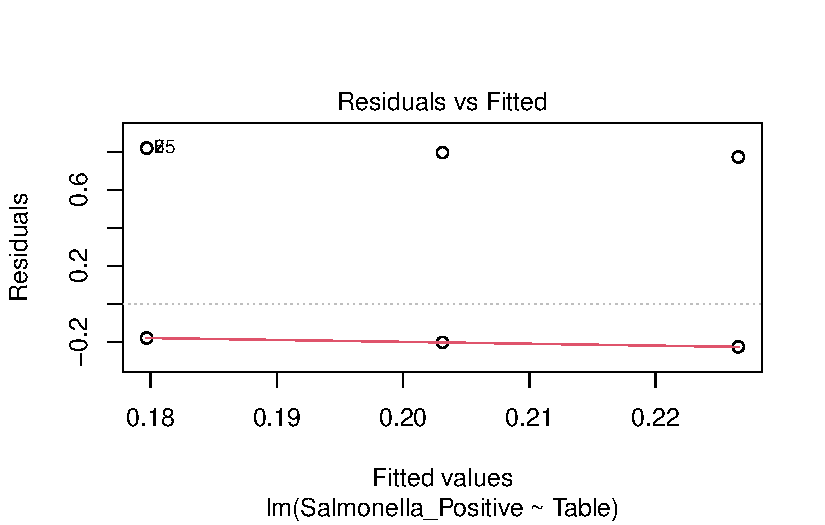
\includegraphics{Supplementary_Material_files/figure-pdf/unnamed-chunk-3-1.pdf}

}

\end{figure}

\begin{figure}[H]

{\centering 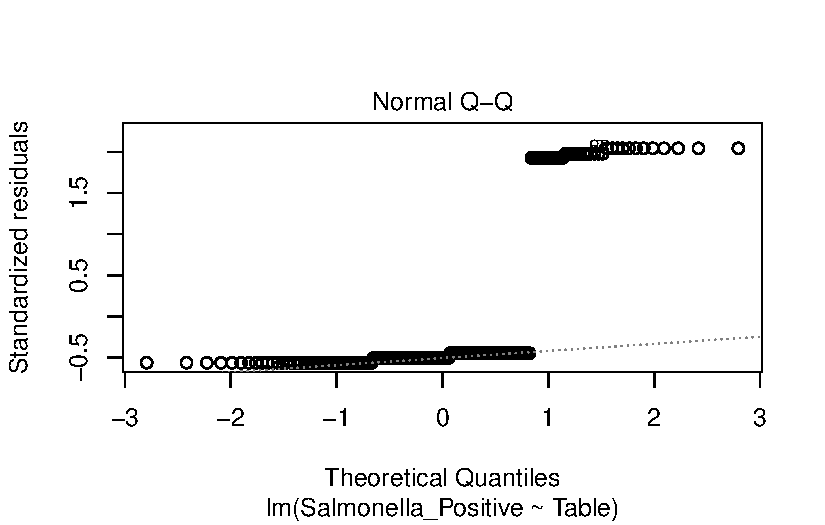
\includegraphics{Supplementary_Material_files/figure-pdf/unnamed-chunk-3-2.pdf}

}

\end{figure}

\begin{figure}[H]

{\centering 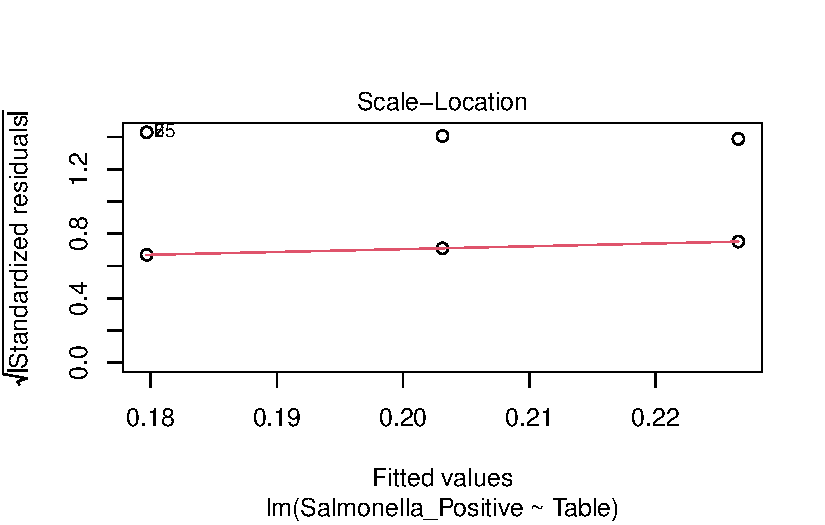
\includegraphics{Supplementary_Material_files/figure-pdf/unnamed-chunk-3-3.pdf}

}

\end{figure}

\begin{figure}[H]

{\centering 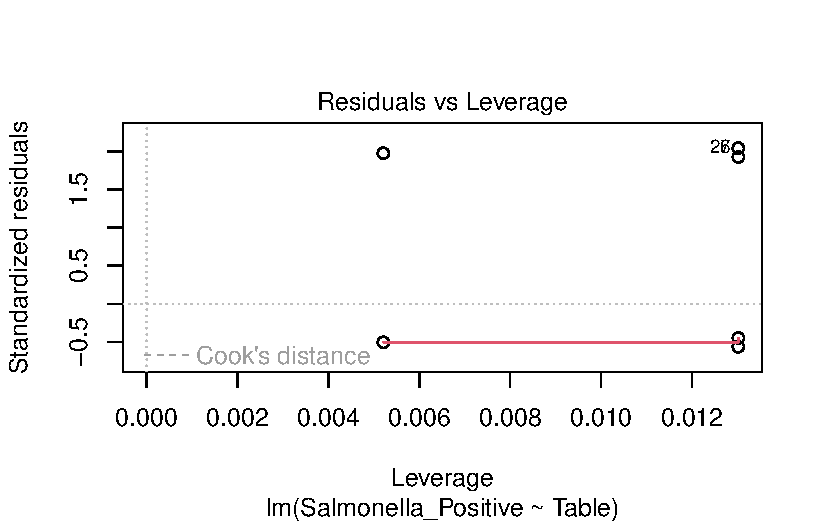
\includegraphics{Supplementary_Material_files/figure-pdf/unnamed-chunk-3-4.pdf}

}

\end{figure}

\begin{Shaded}
\begin{Highlighting}[]
\CommentTok{\# Here we place results from the above fit into a data frame via tidy function}
\NormalTok{lmtable1 }\OtherTok{\textless{}{-}}\NormalTok{ broom}\SpecialCharTok{::}\FunctionTok{tidy}\NormalTok{(lmfit3}\FloatTok{.0}\NormalTok{)}

\CommentTok{\#Let\textquotesingle{}s check out the results}
\FunctionTok{print}\NormalTok{(lmtable1)}
\end{Highlighting}
\end{Shaded}

\begin{verbatim}
# A tibble: 2 x 5
  term        estimate std.error statistic p.value
  <chr>          <dbl>     <dbl>     <dbl>   <dbl>
1 (Intercept)   0.156     0.0771     2.03   0.0442
2 Table         0.0234    0.0357     0.656  0.512 
\end{verbatim}

\begin{Shaded}
\begin{Highlighting}[]
\CommentTok{\#A different way }
\CommentTok{\# I will do the same as above, however, I am now adding persistence pile}
\NormalTok{lmfit2 }\OtherTok{\textless{}{-}} \FunctionTok{lm}\NormalTok{(Salmonella\_Positive}\SpecialCharTok{\textasciitilde{}}\NormalTok{Original\_Persistence\_Pile}\SpecialCharTok{+}\NormalTok{Table, PT\_Data) }
\FunctionTok{plot}\NormalTok{(lmfit2)}
\end{Highlighting}
\end{Shaded}

\begin{figure}[H]

{\centering 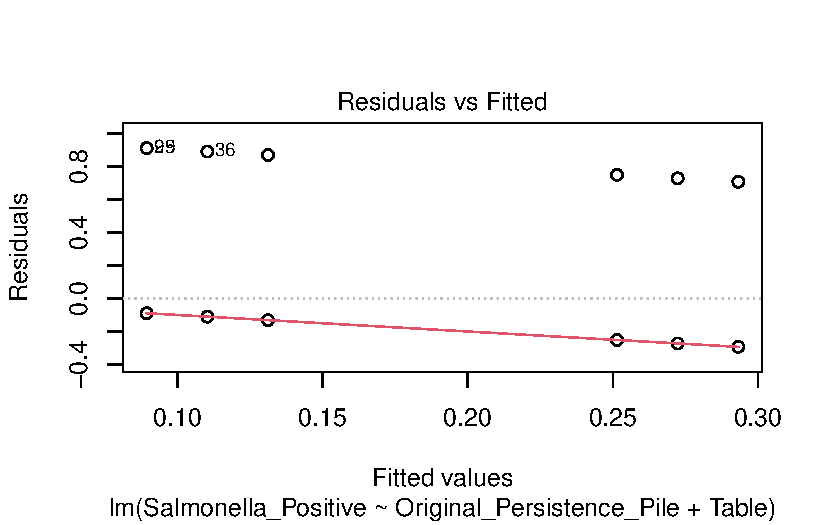
\includegraphics{Supplementary_Material_files/figure-pdf/unnamed-chunk-3-5.pdf}

}

\end{figure}

\begin{figure}[H]

{\centering 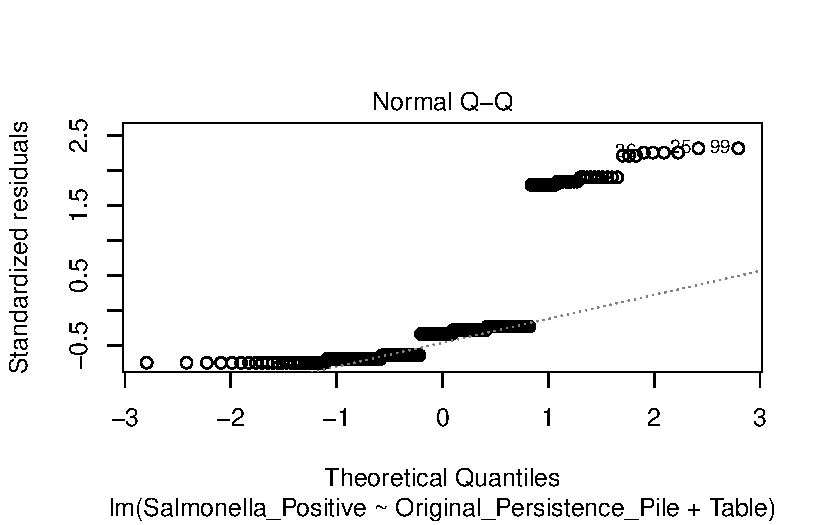
\includegraphics{Supplementary_Material_files/figure-pdf/unnamed-chunk-3-6.pdf}

}

\end{figure}

\begin{figure}[H]

{\centering 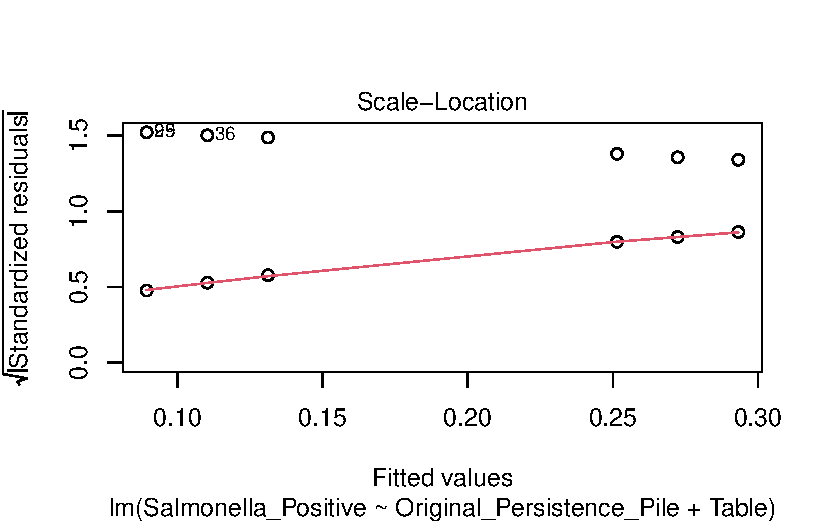
\includegraphics{Supplementary_Material_files/figure-pdf/unnamed-chunk-3-7.pdf}

}

\end{figure}

\begin{figure}[H]

{\centering 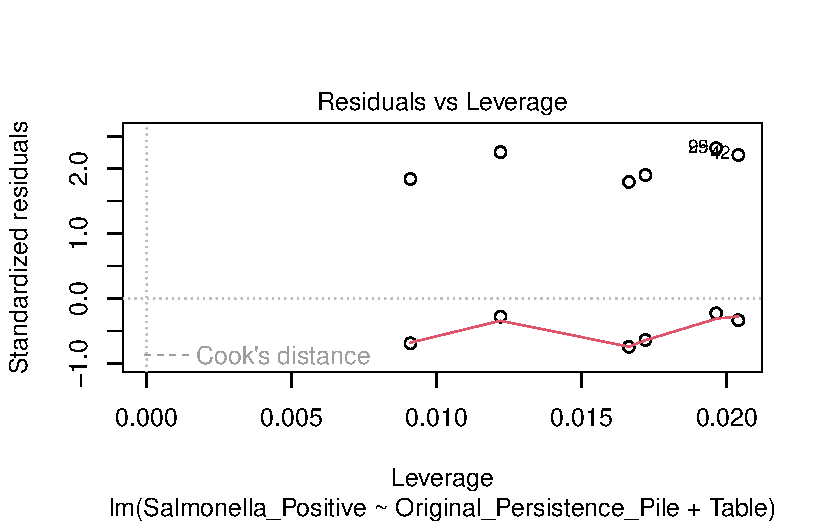
\includegraphics{Supplementary_Material_files/figure-pdf/unnamed-chunk-3-8.pdf}

}

\end{figure}

\begin{Shaded}
\begin{Highlighting}[]
\CommentTok{\# Convert to a data frame via tidy function}
\NormalTok{lmtable2 }\OtherTok{\textless{}{-}}\NormalTok{ broom}\SpecialCharTok{::}\FunctionTok{tidy}\NormalTok{(lmfit2)}

\CommentTok{\#Results}
\FunctionTok{print}\NormalTok{(lmtable2)}
\end{Highlighting}
\end{Shaded}

\begin{verbatim}
# A tibble: 3 x 5
  term                      estimate std.error statistic p.value
  <chr>                        <dbl>     <dbl>     <dbl>   <dbl>
1 (Intercept)                 0.231     0.0803     2.87  0.00456
2 Original_Persistence_Pile  -0.162     0.0579    -2.80  0.00567
3 Table                       0.0209    0.0351     0.596 0.552  
\end{verbatim}

This section is a continuation of what was produced above, however, we
will now be utilizing the Feeder Trial Data

\begin{Shaded}
\begin{Highlighting}[]
\CommentTok{\#Doing the same for FEEDER DATA}
\NormalTok{lmog\_FD}\OtherTok{\textless{}{-}}\FunctionTok{linear\_reg}\NormalTok{() }\SpecialCharTok{\%\textgreater{}\%} 
  \FunctionTok{set\_engine}\NormalTok{(}\StringTok{"lm"}\NormalTok{)}

\NormalTok{model\_lmFD}\OtherTok{\textless{}{-}} \FunctionTok{linear\_reg}\NormalTok{()}

\NormalTok{lmfit\_FD}\OtherTok{\textless{}{-}}\NormalTok{ model\_lmFD }\SpecialCharTok{\%\textgreater{}\%} \CommentTok{\#Training; outcome: Salmonella Pos and Main Predictor Table}
  \FunctionTok{fit}\NormalTok{(Absence\_0\_Presence\_1}\SpecialCharTok{\textasciitilde{}}\NormalTok{Feeder\_number, FD\_Data) }

\NormalTok{lmfit\_FD }\CommentTok{\#Let\textquotesingle{}s view what we just did}
\end{Highlighting}
\end{Shaded}

\begin{verbatim}
parsnip model object


Call:
stats::lm(formula = Absence_0_Presence_1 ~ Feeder_number, data = data)

Coefficients:
  (Intercept)  Feeder_number  
      0.06439        0.01253  
\end{verbatim}

\begin{Shaded}
\begin{Highlighting}[]
\FunctionTok{glimpse}\NormalTok{(lmfit\_FD)}
\end{Highlighting}
\end{Shaded}

\begin{verbatim}
List of 5
 $ lvl    : NULL
 $ spec   :List of 6
  ..$ args                 :List of 2
  .. ..$ penalty: language ~NULL
  .. .. ..- attr(*, ".Environment")=<environment: R_EmptyEnv> 
  .. ..$ mixture: language ~NULL
  .. .. ..- attr(*, ".Environment")=<environment: R_EmptyEnv> 
  ..$ mode                 : chr "regression"
  ..$ user_specified_mode  : logi FALSE
  ..$ method               :List of 3
  .. ..$ libs: chr "stats"
  .. ..$ fit :List of 5
  .. ..$ pred:List of 4
  ..$ engine               : chr "lm"
  ..$ user_specified_engine: logi FALSE
  ..- attr(*, "class")= chr [1:2] "linear_reg" "model_spec"
 $ fit    :List of 12
  ..$ coefficients : Named num [1:2] 0.0644 0.0125
  .. ..- attr(*, "names")= chr [1:2] "(Intercept)" "Feeder_number"
  ..$ residuals    : Named num [1:144] 0.923 0.911 0.898 0.885 0.873 ...
  .. ..- attr(*, "names")= chr [1:144] "1" "2" "3" "4" ...
  ..$ effects      : Named num [1:144] -1.75 0.519 0.77 0.776 0.782 ...
  .. ..- attr(*, "names")= chr [1:144] "(Intercept)" "Feeder_number" "" "" ...
  ..$ rank         : int 2
  ..$ fitted.values: Named num [1:144] 0.0769 0.0895 0.102 0.1145 0.127 ...
  .. ..- attr(*, "names")= chr [1:144] "1" "2" "3" "4" ...
  ..$ assign       : int [1:2] 0 1
  ..$ qr           :List of 5
  .. ..$ qr   : num [1:144, 1:2] -12 0.0833 0.0833 0.0833 0.0833 ...
  .. .. ..- attr(*, "dimnames")=List of 2
  .. .. ..- attr(*, "assign")= int [1:2] 0 1
  .. ..$ qraux: num [1:2] 1.08 1.1
  .. ..$ pivot: int [1:2] 1 2
  .. ..$ tol  : num 1e-07
  .. ..$ rank : int 2
  .. ..- attr(*, "class")= chr "qr"
  ..$ df.residual  : int 142
  ..$ xlevels      : Named list()
  ..$ call         : language stats::lm(formula = Absence_0_Presence_1 ~ Feeder_number, data = data)
  ..$ terms        :Classes 'terms', 'formula'  language Absence_0_Presence_1 ~ Feeder_number
  .. .. ..- attr(*, "variables")= language list(Absence_0_Presence_1, Feeder_number)
  .. .. ..- attr(*, "factors")= int [1:2, 1] 0 1
  .. .. .. ..- attr(*, "dimnames")=List of 2
  .. .. ..- attr(*, "term.labels")= chr "Feeder_number"
  .. .. ..- attr(*, "order")= int 1
  .. .. ..- attr(*, "intercept")= int 1
  .. .. ..- attr(*, "response")= int 1
  .. .. ..- attr(*, ".Environment")=<environment: 0x00000271ddcb4e18> 
  .. .. ..- attr(*, "predvars")= language list(Absence_0_Presence_1, Feeder_number)
  .. .. ..- attr(*, "dataClasses")= Named chr [1:2] "numeric" "numeric"
  .. .. .. ..- attr(*, "names")= chr [1:2] "Absence_0_Presence_1" "Feeder_number"
  ..$ model        :'data.frame':   144 obs. of  2 variables:
  .. ..$ Absence_0_Presence_1: num [1:144] 1 1 1 1 1 1 1 1 1 1 ...
  .. ..$ Feeder_number       : num [1:144] 1 2 3 4 5 6 7 8 9 10 ...
  .. ..- attr(*, "terms")=Classes 'terms', 'formula'  language Absence_0_Presence_1 ~ Feeder_number
  .. .. .. ..- attr(*, "variables")= language list(Absence_0_Presence_1, Feeder_number)
  .. .. .. ..- attr(*, "factors")= int [1:2, 1] 0 1
  .. .. .. .. ..- attr(*, "dimnames")=List of 2
  .. .. .. ..- attr(*, "term.labels")= chr "Feeder_number"
  .. .. .. ..- attr(*, "order")= int 1
  .. .. .. ..- attr(*, "intercept")= int 1
  .. .. .. ..- attr(*, "response")= int 1
  .. .. .. ..- attr(*, ".Environment")=<environment: 0x00000271ddcb4e18> 
  .. .. .. ..- attr(*, "predvars")= language list(Absence_0_Presence_1, Feeder_number)
  .. .. .. ..- attr(*, "dataClasses")= Named chr [1:2] "numeric" "numeric"
  .. .. .. .. ..- attr(*, "names")= chr [1:2] "Absence_0_Presence_1" "Feeder_number"
  ..- attr(*, "class")= chr "lm"
 $ preproc:List of 1
  ..$ y_var: chr "Absence_0_Presence_1"
 $ elapsed:List of 1
  ..$ elapsed: num NA
 - attr(*, "class")= chr [1:2] "_lm" "model_fit"
\end{verbatim}

\begin{Shaded}
\begin{Highlighting}[]
\FunctionTok{tidy}\NormalTok{(lmfit\_FD) }\CommentTok{\#We can use the tidy() function to produce the output/ summary statistics}
\end{Highlighting}
\end{Shaded}

\begin{verbatim}
# A tibble: 2 x 5
  term          estimate std.error statistic p.value
  <chr>            <dbl>     <dbl>     <dbl>   <dbl>
1 (Intercept)     0.0644   0.0627       1.03   0.306
2 Feeder_number   0.0125   0.00852      1.47   0.143
\end{verbatim}

\begin{Shaded}
\begin{Highlighting}[]
\FunctionTok{plot\_summs}\NormalTok{(lmfit\_FD)}
\end{Highlighting}
\end{Shaded}

\begin{figure}[H]

{\centering 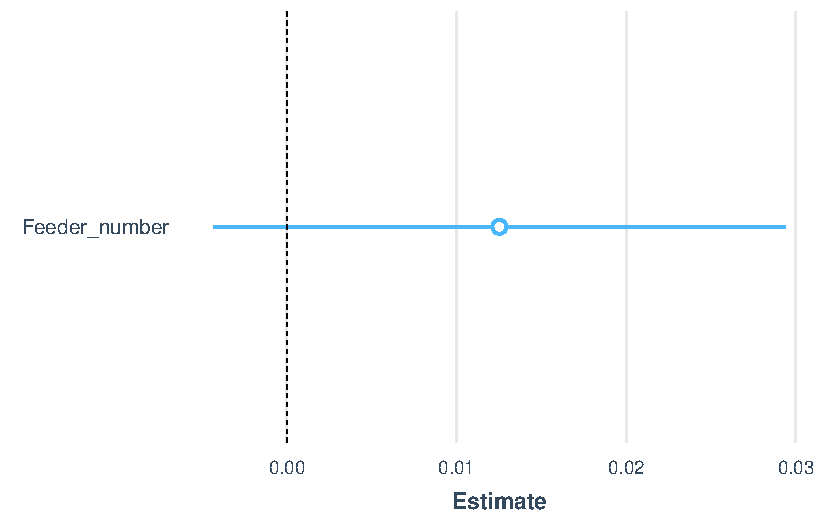
\includegraphics{Supplementary_Material_files/figure-pdf/unnamed-chunk-4-1.pdf}

}

\end{figure}

\begin{Shaded}
\begin{Highlighting}[]
\CommentTok{\#Checking model performance: FEEDER}
\FunctionTok{check\_model}\NormalTok{(lmfit\_FD}\SpecialCharTok{$}\NormalTok{fit)}
\end{Highlighting}
\end{Shaded}

\begin{figure}[H]

{\centering 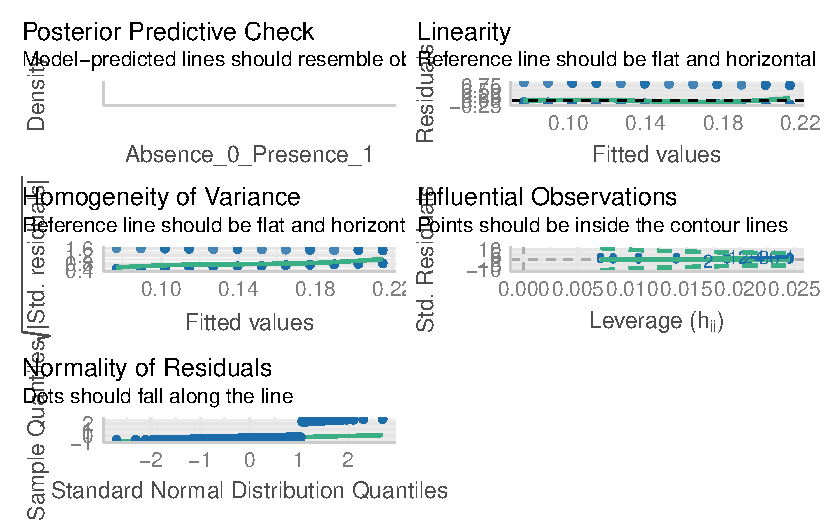
\includegraphics{Supplementary_Material_files/figure-pdf/unnamed-chunk-4-2.pdf}

}

\end{figure}

\textbf{Time to Event Analysis: Picnic Table Trial}

\begin{Shaded}
\begin{Highlighting}[]
\NormalTok{PT\_Data\_TTE}\OtherTok{\textless{}{-}} \CommentTok{\#First let\textquotesingle{}s format the dates }
\NormalTok{  PT\_Data }\SpecialCharTok{\%\textgreater{}\%} 
  \FunctionTok{mutate}\NormalTok{(}
    \AttributeTok{Date=} \FunctionTok{ymd}\NormalTok{(Date))}

\NormalTok{PT\_Data\_TTE}\SpecialCharTok{$}\NormalTok{Date}\OtherTok{\textless{}{-}} \FunctionTok{as.numeric}\NormalTok{(PT\_Data\_TTE}\SpecialCharTok{$}\NormalTok{Date) }\CommentTok{\#Let\textquotesingle{}s make these numeric}

\NormalTok{PT\_Data\_TTE }\OtherTok{\textless{}{-}} \CommentTok{\#I want to add a column displaying time between events (by day)}
\NormalTok{  PT\_Data\_TTE }\SpecialCharTok{\%\textgreater{}\%}
  \FunctionTok{mutate}\NormalTok{(}
    \AttributeTok{os\_day=} \FunctionTok{as.duration}\NormalTok{(Date)}\SpecialCharTok{/}\FunctionTok{ddays}\NormalTok{(}\DecValTok{1}\NormalTok{))}

\NormalTok{PT\_Data\_TTE}\SpecialCharTok{$}\NormalTok{os\_day}\OtherTok{\textless{}{-}} \FunctionTok{as.numeric}\NormalTok{(PT\_Data\_TTE}\SpecialCharTok{$}\NormalTok{os\_day) }\CommentTok{\#Again let\textquotesingle{}s make sure our new column is in the proper format}

\NormalTok{surv1}\OtherTok{\textless{}{-}} \FunctionTok{Surv}\NormalTok{(PT\_Data\_TTE}\SpecialCharTok{$}\NormalTok{Date,PT\_Data\_TTE}\SpecialCharTok{$}\NormalTok{Salmonella\_Positive) }

\CommentTok{\#Let\textquotesingle{}s visualize!}
\NormalTok{sfit1}\OtherTok{\textless{}{-}} \FunctionTok{survfit}\NormalTok{(}\FunctionTok{Surv}\NormalTok{(Date, Salmonella\_Positive) }\SpecialCharTok{\textasciitilde{}}  \DecValTok{1}\NormalTok{, }\AttributeTok{data=}\NormalTok{PT\_Data\_TTE)  }\SpecialCharTok{\%\textgreater{}\%} 
  \FunctionTok{ggsurvfit}\NormalTok{() }\SpecialCharTok{+} 
  \FunctionTok{labs}\NormalTok{(}
    \AttributeTok{x =} \StringTok{"Days"}\NormalTok{,}
    \AttributeTok{y =} \StringTok{"Overall Salmonella Persistence"}\NormalTok{) }\SpecialCharTok{+} \CommentTok{\#Let\textquotesingle{}s add some labels}
  \FunctionTok{add\_confidence\_interval}\NormalTok{() }\SpecialCharTok{+}
  \FunctionTok{add\_risktable}\NormalTok{()}

\CommentTok{\#I am not confident with this graphic so I will include this in my supplemental section}
\end{Highlighting}
\end{Shaded}

\begin{Shaded}
\begin{Highlighting}[]
\FunctionTok{glimpse}\NormalTok{(PT\_Data)}
\end{Highlighting}
\end{Shaded}

\begin{verbatim}
Rows: 192
Columns: 7
$ ID                        <chr> "DPT1Q1 PER 1-2-2020", "DPT1Q2 PER 1-2-2020"~
$ Date                      <dttm> 2020-01-02, 2020-01-02, 2020-01-02, 2020-01~
$ Table                     <dbl> 1, 1, 1, 1, 1, 1, 1, 1, 2, 2, 2, 2, 2, 2, 2,~
$ Quadrant                  <dbl> 1, 2, 3, 4, 1, 2, 3, 4, 1, 2, 3, 4, 1, 2, 3,~
$ Sample_Type               <chr> "Persistence", "Persistence", "Persistence",~
$ Original_Persistence_Pile <dbl> 0, 0, 0, 0, 0, 0, 0, 0, 0, 0, 0, 0, 0, 0, 0,~
$ Salmonella_Positive       <dbl> 0, 0, 0, 0, 0, 1, 1, 0, 0, 0, 0, 1, 1, 0, 0,~
\end{verbatim}

\begin{Shaded}
\begin{Highlighting}[]
\NormalTok{PT\_Data }\OtherTok{=}\NormalTok{ PT\_Data }\SpecialCharTok{\%\textgreater{}\%} 
 \FunctionTok{mutate}\NormalTok{(}
  \AttributeTok{salmonella\_crr=} \FunctionTok{case\_when}\NormalTok{(}
\NormalTok{   Salmonella\_Positive }\SpecialCharTok{==}  \DecValTok{0}\SpecialCharTok{\textasciitilde{}}\DecValTok{1}\NormalTok{,}
\NormalTok{    Salmonella\_Positive }\SpecialCharTok{==} \DecValTok{1}\SpecialCharTok{\textasciitilde{}}\DecValTok{1}\NormalTok{,}
     \ConstantTok{TRUE} \SpecialCharTok{\textasciitilde{}} \DecValTok{1}\NormalTok{))}

\NormalTok{dependent\_crr}\OtherTok{=} \StringTok{"Surv(Date, salmonella\_crr)"}
\NormalTok{explanatory}\OtherTok{=} \FunctionTok{c}\NormalTok{(}\StringTok{"Table"}\NormalTok{, }\StringTok{"Quadrant"}\NormalTok{, }\StringTok{"Sample\_Type"}\NormalTok{)}

\NormalTok{PT\_Data}\SpecialCharTok{$}\NormalTok{Date}\OtherTok{\textless{}{-}} \FunctionTok{as.numeric}\NormalTok{(PT\_Data}\SpecialCharTok{$}\NormalTok{Date)}

\NormalTok{PT\_Data }\SpecialCharTok{\%\textgreater{}\%} \FunctionTok{finalfit}\NormalTok{(dependent\_crr, explanatory)}
\end{Highlighting}
\end{Shaded}

\begin{verbatim}
 Dependent: Surv(Date, salmonella_crr)                   all
                                 Table           1 64 (33.3)
                                                 2 64 (33.3)
                                                 3 64 (33.3)
                              Quadrant           1 48 (25.0)
                                                 2 48 (25.0)
                                                 3 48 (25.0)
                                                 4 48 (25.0)
                           Sample_Type Persistence 96 (50.0)
                                            Pooled 96 (50.0)
          HR (univariable)        HR (multivariable)
                         -                         -
 1.00 (0.71-1.41, p=1.000) 1.00 (0.71-1.41, p=1.000)
 1.00 (0.71-1.41, p=1.000) 1.00 (0.71-1.41, p=1.000)
                         -                         -
 1.00 (0.67-1.49, p=1.000) 1.00 (0.67-1.49, p=1.000)
 1.00 (0.67-1.49, p=1.000) 1.00 (0.67-1.49, p=1.000)
 1.00 (0.67-1.49, p=1.000) 1.00 (0.67-1.49, p=1.000)
                         -                         -
 1.00 (0.75-1.33, p=1.000) 1.00 (0.75-1.33, p=1.000)
\end{verbatim}

\begin{Shaded}
\begin{Highlighting}[]
\NormalTok{PT\_Data }\SpecialCharTok{\%\textgreater{}\%} 
   \FunctionTok{finalfit}\NormalTok{(dependent\_crr, explanatory, }\AttributeTok{add\_dependent\_label =} \ConstantTok{FALSE}\NormalTok{) }\SpecialCharTok{\%\textgreater{}\%} 
    \FunctionTok{rename}\NormalTok{(}\StringTok{"Overall survival"} \OtherTok{=}\NormalTok{ label) }\SpecialCharTok{\%\textgreater{}\%} 
    \FunctionTok{rename}\NormalTok{(}\StringTok{" "} \OtherTok{=}\NormalTok{ levels) }\SpecialCharTok{\%\textgreater{}\%} 
    \FunctionTok{rename}\NormalTok{(}\StringTok{"  "} \OtherTok{=}\NormalTok{ all) }
\end{Highlighting}
\end{Shaded}

\begin{verbatim}
 Overall survival                                HR (univariable)
            Table           1 64 (33.3)                         -
                            2 64 (33.3) 1.00 (0.71-1.41, p=1.000)
                            3 64 (33.3) 1.00 (0.71-1.41, p=1.000)
         Quadrant           1 48 (25.0)                         -
                            2 48 (25.0) 1.00 (0.67-1.49, p=1.000)
                            3 48 (25.0) 1.00 (0.67-1.49, p=1.000)
                            4 48 (25.0) 1.00 (0.67-1.49, p=1.000)
      Sample_Type Persistence 96 (50.0)                         -
                       Pooled 96 (50.0) 1.00 (0.75-1.33, p=1.000)
        HR (multivariable)
                         -
 1.00 (0.71-1.41, p=1.000)
 1.00 (0.71-1.41, p=1.000)
                         -
 1.00 (0.67-1.49, p=1.000)
 1.00 (0.67-1.49, p=1.000)
 1.00 (0.67-1.49, p=1.000)
                         -
 1.00 (0.75-1.33, p=1.000)
\end{verbatim}

\begin{Shaded}
\begin{Highlighting}[]
\FunctionTok{survfit}\NormalTok{(}\FunctionTok{Surv}\NormalTok{(Date, Salmonella\_Positive)}\SpecialCharTok{\textasciitilde{}}\DecValTok{1}\NormalTok{, }\AttributeTok{data=}\NormalTok{PT\_Data)}
\end{Highlighting}
\end{Shaded}

\begin{verbatim}
Call: survfit(formula = Surv(Date, Salmonella_Positive) ~ 1, data = PT_Data)

       n events median 0.95LCL 0.95UCL
[1,] 192     39     NA      NA      NA
\end{verbatim}

\begin{Shaded}
\begin{Highlighting}[]
\NormalTok{PT\_MedSurv}\OtherTok{\textless{}{-}}\NormalTok{PT\_Data }\SpecialCharTok{\%\textgreater{}\%}
 \FunctionTok{filter}\NormalTok{(salmonella\_crr}\SpecialCharTok{==}\DecValTok{1}\NormalTok{) }\SpecialCharTok{\%\textgreater{}\%}
  \FunctionTok{summarize}\NormalTok{(}\AttributeTok{median\_surv=}\FunctionTok{median}\NormalTok{(Date))}

\NormalTok{PT\_MedSurv }\OtherTok{\textless{}{-}}\NormalTok{ ((PT\_MedSurv)}\SpecialCharTok{/}\DecValTok{31556952000}\NormalTok{)}\SpecialCharTok{*}\DecValTok{100}

\NormalTok{PT\_Surv\_Table}\OtherTok{\textless{}{-}} \FunctionTok{gt}\NormalTok{(PT\_MedSurv) }\SpecialCharTok{\%\textgreater{}\%}
   \FunctionTok{tab\_header}\NormalTok{(}
    \AttributeTok{title =} \StringTok{"Median Survival of Salmonella"}\NormalTok{,}
    \AttributeTok{subtitle =}\NormalTok{ (}\StringTok{"01/02/2020 to 01/09/2020"}\NormalTok{)) }\SpecialCharTok{\%\textgreater{}\%}
  \FunctionTok{cols\_label}\NormalTok{(}
    \AttributeTok{median\_surv=} \StringTok{"Median Salmonella Survival (days)"}\NormalTok{) }

\NormalTok{PT\_Surv\_Table }\CommentTok{\# persistence seems to be roughly 5 days}
\end{Highlighting}
\end{Shaded}

\begin{longtable}{r}
\caption*{
{\large Median Survival of Salmonella} \\ 
{\small 01/02/2020 to 01/09/2020}
} \\ 
\toprule
Median Salmonella Survival (days) \\ 
\midrule
5.001198 \\ 
\bottomrule
\end{longtable}

\textbf{Time to Event Analysis: Feeder Trial}

\begin{Shaded}
\begin{Highlighting}[]
\NormalTok{FD\_Data\_TTE}\OtherTok{\textless{}{-}} \CommentTok{\#First let\textquotesingle{}s format the dates }
\NormalTok{  FD\_Data }\SpecialCharTok{\%\textgreater{}\%} 
  \FunctionTok{mutate}\NormalTok{(}
    \AttributeTok{Date=} \FunctionTok{ymd}\NormalTok{(Collection\_Date))}

\NormalTok{FD\_Data\_TTE}\SpecialCharTok{$}\NormalTok{Collection\_Date}\OtherTok{\textless{}{-}} \FunctionTok{as.numeric}\NormalTok{(FD\_Data\_TTE}\SpecialCharTok{$}\NormalTok{Collection\_Date) }\CommentTok{\#Let\textquotesingle{}s make these numeric}

\NormalTok{FD\_Data\_TTE }\OtherTok{\textless{}{-}} \CommentTok{\#I want to add a column displaying time between events (by day)}
\NormalTok{  FD\_Data\_TTE }\SpecialCharTok{\%\textgreater{}\%}
  \FunctionTok{mutate}\NormalTok{(}
    \AttributeTok{os\_day=} \FunctionTok{as.duration}\NormalTok{(Collection\_Date)}\SpecialCharTok{/}\FunctionTok{ddays}\NormalTok{(}\DecValTok{1}\NormalTok{))}

\NormalTok{FD\_Data\_TTE}\SpecialCharTok{$}\NormalTok{os\_day}\OtherTok{\textless{}{-}} \FunctionTok{as.numeric}\NormalTok{(FD\_Data\_TTE}\SpecialCharTok{$}\NormalTok{os\_day) }\CommentTok{\#Again let\textquotesingle{}s make sure our new column is in the proper format}

\NormalTok{surv1\_FD}\OtherTok{\textless{}{-}} \FunctionTok{Surv}\NormalTok{(FD\_Data\_TTE}\SpecialCharTok{$}\NormalTok{Collection\_Date,FD\_Data\_TTE}\SpecialCharTok{$}\NormalTok{Absence\_0\_Presence\_1) }

\CommentTok{\#Let\textquotesingle{}s visualize!}
\NormalTok{sfit1}\OtherTok{\textless{}{-}} \FunctionTok{survfit}\NormalTok{(}\FunctionTok{Surv}\NormalTok{(Collection\_Date, Absence\_0\_Presence\_1) }\SpecialCharTok{\textasciitilde{}}  \DecValTok{1}\NormalTok{, }\AttributeTok{data=}\NormalTok{FD\_Data\_TTE)  }\SpecialCharTok{\%\textgreater{}\%} 
  \FunctionTok{ggsurvfit}\NormalTok{() }\SpecialCharTok{+} 
  \FunctionTok{labs}\NormalTok{(}
    \AttributeTok{x =} \StringTok{"Days"}\NormalTok{,}
    \AttributeTok{y =} \StringTok{"Overall Salmonella Persistence"}\NormalTok{) }\SpecialCharTok{+} \CommentTok{\#Let\textquotesingle{}s add some labels}
  \FunctionTok{add\_confidence\_interval}\NormalTok{() }\SpecialCharTok{+}
  \FunctionTok{add\_risktable}\NormalTok{()}

\NormalTok{sfit1}
\end{Highlighting}
\end{Shaded}

\begin{figure}[H]

{\centering 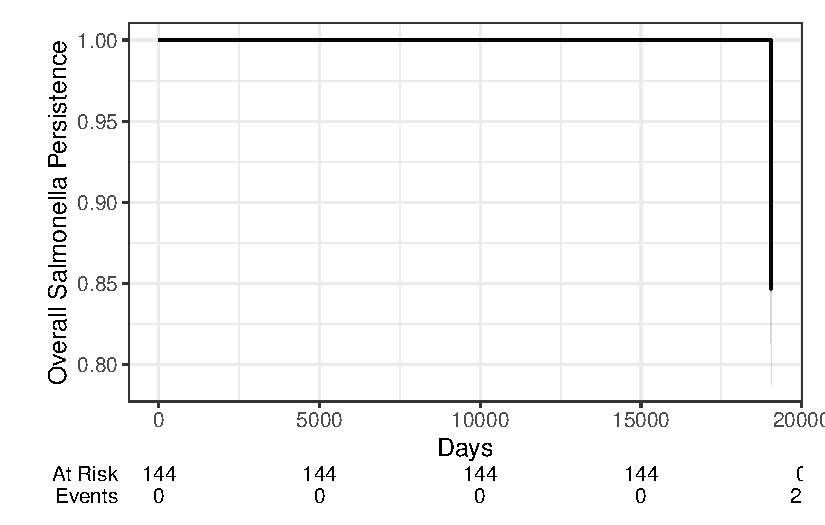
\includegraphics{Supplementary_Material_files/figure-pdf/unnamed-chunk-7-1.pdf}

}

\end{figure}

\begin{Shaded}
\begin{Highlighting}[]
\NormalTok{FD\_Data }\OtherTok{=}\NormalTok{ FD\_Data }\SpecialCharTok{\%\textgreater{}\%} 
 \FunctionTok{mutate}\NormalTok{(}
  \AttributeTok{salmonella\_crr=} \FunctionTok{case\_when}\NormalTok{(}
\NormalTok{   Absence\_0\_Presence\_1 }\SpecialCharTok{==}  \DecValTok{0}\SpecialCharTok{\textasciitilde{}}\DecValTok{1}\NormalTok{,}
\NormalTok{    Absence\_0\_Presence\_1 }\SpecialCharTok{==} \DecValTok{1}\SpecialCharTok{\textasciitilde{}}\DecValTok{1}\NormalTok{,}
     \ConstantTok{TRUE} \SpecialCharTok{\textasciitilde{}} \DecValTok{1}\NormalTok{))}

\NormalTok{dependent\_crr}\OtherTok{=} \StringTok{"Surv(Collection\_Date, salmonella\_crr)"}
\NormalTok{explanatory}\OtherTok{=} \FunctionTok{c}\NormalTok{(}\StringTok{"Feeder\_Type"}\NormalTok{)}

\NormalTok{FD\_Data}\SpecialCharTok{$}\NormalTok{Collection\_Date}\OtherTok{\textless{}{-}} \FunctionTok{as.numeric}\NormalTok{(FD\_Data}\SpecialCharTok{$}\NormalTok{Collection\_Date)}

\NormalTok{FD\_Data }\SpecialCharTok{\%\textgreater{}\%} \FunctionTok{finalfit}\NormalTok{(dependent\_crr, explanatory)}
\end{Highlighting}
\end{Shaded}

\begin{verbatim}
 Dependent: Surv(Collection_Date, salmonella_crr)                      all
                                      Feeder_Type        Plastic 36 (25.0)
                                                  Plastic_coated 36 (25.0)
                                                            Wood 36 (25.0)
                                                     Wood_coated 36 (25.0)
          HR (univariable)        HR (multivariable)
                         -                         -
 1.00 (0.63-1.59, p=1.000) 1.00 (0.63-1.59, p=1.000)
 1.00 (0.63-1.59, p=1.000) 1.00 (0.63-1.59, p=1.000)
 1.00 (0.63-1.59, p=1.000) 1.00 (0.63-1.59, p=1.000)
\end{verbatim}

\begin{Shaded}
\begin{Highlighting}[]
\NormalTok{FD\_Data }\SpecialCharTok{\%\textgreater{}\%} 
   \FunctionTok{finalfit}\NormalTok{(dependent\_crr, explanatory, }\AttributeTok{add\_dependent\_label =} \ConstantTok{FALSE}\NormalTok{) }\SpecialCharTok{\%\textgreater{}\%} 
    \FunctionTok{rename}\NormalTok{(}\StringTok{"Overall survival"} \OtherTok{=}\NormalTok{ label) }\SpecialCharTok{\%\textgreater{}\%} 
    \FunctionTok{rename}\NormalTok{(}\StringTok{" "} \OtherTok{=}\NormalTok{ levels) }\SpecialCharTok{\%\textgreater{}\%} 
    \FunctionTok{rename}\NormalTok{(}\StringTok{"  "} \OtherTok{=}\NormalTok{ all) }
\end{Highlighting}
\end{Shaded}

\begin{verbatim}
 Overall survival                                   HR (univariable)
      Feeder_Type        Plastic 36 (25.0)                         -
                  Plastic_coated 36 (25.0) 1.00 (0.63-1.59, p=1.000)
                            Wood 36 (25.0) 1.00 (0.63-1.59, p=1.000)
                     Wood_coated 36 (25.0) 1.00 (0.63-1.59, p=1.000)
        HR (multivariable)
                         -
 1.00 (0.63-1.59, p=1.000)
 1.00 (0.63-1.59, p=1.000)
 1.00 (0.63-1.59, p=1.000)
\end{verbatim}

\begin{Shaded}
\begin{Highlighting}[]
\FunctionTok{survfit}\NormalTok{(}\FunctionTok{Surv}\NormalTok{(Collection\_Date, Absence\_0\_Presence\_1)}\SpecialCharTok{\textasciitilde{}}\DecValTok{1}\NormalTok{, }\AttributeTok{data=}\NormalTok{FD\_Data)}
\end{Highlighting}
\end{Shaded}

\begin{verbatim}
Call: survfit(formula = Surv(Collection_Date, Absence_0_Presence_1) ~ 
    1, data = FD_Data)

       n events median 0.95LCL 0.95UCL
[1,] 144     21     NA      NA      NA
\end{verbatim}

\begin{Shaded}
\begin{Highlighting}[]
\NormalTok{FD\_MedSurv}\OtherTok{\textless{}{-}}\NormalTok{FD\_Data }\SpecialCharTok{\%\textgreater{}\%}
 \FunctionTok{filter}\NormalTok{(salmonella\_crr}\SpecialCharTok{==}\DecValTok{1}\NormalTok{) }\SpecialCharTok{\%\textgreater{}\%}
  \FunctionTok{summarize}\NormalTok{(}\AttributeTok{median\_surv=}\FunctionTok{median}\NormalTok{(Collection\_Date))}

\NormalTok{FD\_MedSurv }\OtherTok{\textless{}{-}}\NormalTok{ ((FD\_MedSurv)}\SpecialCharTok{/}\DecValTok{604800}\NormalTok{)}\SpecialCharTok{*}\DecValTok{100} \CommentTok{\#Persistence seems to be roughly 3 days for the FD}

\NormalTok{FD\_Surv\_Table}\OtherTok{\textless{}{-}} \FunctionTok{gt}\NormalTok{(FD\_MedSurv) }\SpecialCharTok{\%\textgreater{}\%}
   \FunctionTok{tab\_header}\NormalTok{(}
    \AttributeTok{title =} \StringTok{"Median Survival of Salmonella"}\NormalTok{,}
    \AttributeTok{subtitle =}\NormalTok{ (}\StringTok{"02/22/2022 to 03/14/2022"}\NormalTok{)) }\SpecialCharTok{\%\textgreater{}\%}
  \FunctionTok{cols\_label}\NormalTok{(}
    \AttributeTok{median\_surv=} \StringTok{"Median Salmonella Survival (days)"}\NormalTok{) }

\NormalTok{FD\_Surv\_Table }\CommentTok{\# seems to be roughly 3 days}
\end{Highlighting}
\end{Shaded}

\begin{longtable}{r}
\caption*{
{\large Median Survival of Salmonella} \\ 
{\small 02/22/2022 to 03/14/2022}
} \\ 
\toprule
Median Salmonella Survival (days) \\ 
\midrule
3.149884 \\ 
\bottomrule
\end{longtable}

\textbf{Cox regression: Picnic Table Trial}

\begin{Shaded}
\begin{Highlighting}[]
\NormalTok{PT\_Data}\SpecialCharTok{$}\NormalTok{Date}\OtherTok{\textless{}{-}} \FunctionTok{as.numeric}\NormalTok{(PT\_Data}\SpecialCharTok{$}\NormalTok{Date)}

\FunctionTok{coxph}\NormalTok{(}\FunctionTok{Surv}\NormalTok{(Date, Salmonella\_Positive) }\SpecialCharTok{\textasciitilde{}}\NormalTok{ Sample\_Type, PT\_Data)}
\end{Highlighting}
\end{Shaded}

\begin{verbatim}
Call:
coxph(formula = Surv(Date, Salmonella_Positive) ~ Sample_Type, 
    data = PT_Data)

                    coef exp(coef) se(coef)     z      p
Sample_TypePooled 0.8344    2.3034   0.3470 2.405 0.0162

Likelihood ratio test=6.28  on 1 df, p=0.01224
n= 192, number of events= 39 
\end{verbatim}

\begin{Shaded}
\begin{Highlighting}[]
\NormalTok{CR\_PT1}\OtherTok{\textless{}{-}}\FunctionTok{coxph}\NormalTok{(}\FunctionTok{Surv}\NormalTok{(Date, Salmonella\_Positive) }\SpecialCharTok{\textasciitilde{}}\NormalTok{ Sample\_Type, PT\_Data) }\SpecialCharTok{\%\textgreater{}\%}
  \FunctionTok{tbl\_regression}\NormalTok{(}\AttributeTok{exp=}\ConstantTok{TRUE}\NormalTok{)}

\NormalTok{CR\_PT1}
\end{Highlighting}
\end{Shaded}

\begin{verbatim}
Table printed with `knitr::kable()`, not {gt}. Learn why at
https://www.danieldsjoberg.com/gtsummary/articles/rmarkdown.html
To suppress this message, include `message = FALSE` in code chunk header.
\end{verbatim}

\begin{longtable}[]{@{}lccc@{}}
\toprule()
\textbf{Characteristic} & \textbf{HR} & \textbf{95\% CI} &
\textbf{p-value} \\
\midrule()
\endhead
Sample\_Type & & & \\
Persistence & --- & --- & \\
Pooled & 2.30 & 1.17, 4.55 & 0.016 \\
\bottomrule()
\end{longtable}

\textbf{Cox regression: Feeder Trial}

\begin{Shaded}
\begin{Highlighting}[]
\NormalTok{FD\_Data}\SpecialCharTok{$}\NormalTok{Collection\_Date}\OtherTok{\textless{}{-}} \FunctionTok{as.numeric}\NormalTok{(FD\_Data}\SpecialCharTok{$}\NormalTok{Collection\_Date)}

\FunctionTok{coxph}\NormalTok{(}\FunctionTok{Surv}\NormalTok{(Collection\_Date, Absence\_0\_Presence\_1) }\SpecialCharTok{\textasciitilde{}}\NormalTok{ Feeder\_Type, FD\_Data)}
\end{Highlighting}
\end{Shaded}

\begin{verbatim}
Call:
coxph(formula = Surv(Collection_Date, Absence_0_Presence_1) ~ 
    Feeder_Type, data = FD_Data)

                             coef exp(coef) se(coef)      z     p
Feeder_TypePlastic_coated  0.2918    1.3389   0.5401  0.540 0.589
Feeder_TypeWood           -0.4111    0.6629   0.6455 -0.637 0.524
Feeder_TypeWood_coated    -0.6999    0.4966   0.7071 -0.990 0.322

Likelihood ratio test=2.88  on 3 df, p=0.4112
n= 144, number of events= 21 
\end{verbatim}

\begin{Shaded}
\begin{Highlighting}[]
\NormalTok{CR\_FD1}\OtherTok{\textless{}{-}} \FunctionTok{coxph}\NormalTok{(}\FunctionTok{Surv}\NormalTok{(Collection\_Date, Absence\_0\_Presence\_1) }\SpecialCharTok{\textasciitilde{}}\NormalTok{ Feeder\_Type, FD\_Data) }\SpecialCharTok{\%\textgreater{}\%}
  \FunctionTok{tbl\_regression}\NormalTok{(}\AttributeTok{exp=}\ConstantTok{TRUE}\NormalTok{)}

\NormalTok{CR\_FD1}
\end{Highlighting}
\end{Shaded}

\begin{verbatim}
Table printed with `knitr::kable()`, not {gt}. Learn why at
https://www.danieldsjoberg.com/gtsummary/articles/rmarkdown.html
To suppress this message, include `message = FALSE` in code chunk header.
\end{verbatim}

\begin{longtable}[]{@{}lccc@{}}
\toprule()
\textbf{Characteristic} & \textbf{HR} & \textbf{95\% CI} &
\textbf{p-value} \\
\midrule()
\endhead
Feeder\_Type & & & \\
Plastic & --- & --- & \\
Plastic\_coated & 1.34 & 0.46, 3.86 & 0.6 \\
Wood & 0.66 & 0.19, 2.35 & 0.5 \\
Wood\_coated & 0.50 & 0.12, 1.99 & 0.3 \\
\bottomrule()
\end{longtable}

\begin{Shaded}
\begin{Highlighting}[]
\NormalTok{CR\_FD1}\SpecialCharTok{\%\textgreater{}\%}
  \FunctionTok{saveRDS}\NormalTok{(}\FunctionTok{here}\NormalTok{(}\StringTok{"4. Results"}\NormalTok{, }\StringTok{"FD\_Cox.rds"}\NormalTok{))}
\end{Highlighting}
\end{Shaded}




\end{document}
